\documentclass[a4paper,english]{G2-105}
\usepackage[T1]{fontenc}
\usepackage{multirow}
\usepackage{graphicx}

\VSTUSetDocumentNumbersPrefix{}
\VSTUSetDocumentCode{ВРБ-40-461-806-10.19-09.03.04-02-15}
\VSTUSetDocumentTypeDative{выпускной работе бакалавра}
%\VSTUSetDocumentTypeGenitive{выпускную работу бакалавра}
\VSTUSetInitialData{задание, выданное научным руководителем с кафедры ПОАС,
утвержденное приказом ректора}

\begin{document}
\VSTUMakeCenteredTOC
\VSTUSetOrder{1529–ст}{17}{октября}{2014}
\VSTUSetFaculty{Электроники и вычислительной техники}
\VSTUSetDepartment{Программное обеспечение автоматизированных систем}
\VSTUSetDepartmentCode{10.19}
\VSTUSetDirection{230100.62 Программная инженерия}
\VSTUSetHeadOfDepartment{Зав. кафедрой ПОАС}{д.т.н., проф.}{А. М. Дворянкин}{Дворянкин Александр Михайлович}
\VSTUSetDocumentNumbersPrefix{А.}
\VSTUSetDirector{доц. каф. ПОАС}{к.т.н.}{О. А. Сычев}{Сычев Олег Александрович}
\VSTUSetStandardsAdviser{ст. преп. каф. ПОАС}{}{О. Н. Ляпина}{Ляпина Ольга Николаевна}
\VSTUSetStudent{ПрИн-466}{В. А. Клевцов}{Клевцов Вадим Александрович}
\VSTUSetTitle{Поддержка перечислений для языка С++ в типе вопроса CorrectWriting}
\VSTUSetTitleEng{Support enumerations for C++ in the question type CorrectWriting}
\abstract{Аннотация}
\par Документ представляет собой техническое задание к выпускной работе бакалавра на тему «Поддержка перечислений для языка С++ в типе вопроса CorrectWriting», выполненную студентом группы ПрИн-466, Клевцовым Вадимом Александровичем.
\par В данной работе были разработаны требования к разрабатываемому модулю, его ограничения на его работу.
\par Объём технического задания составил \totalpages~страниц и включает \totalfigures~рисунка и \totaltables~таблицы. 
\par Ключевые слова: система дистанционного образования, Moodle, мудл, CorrectWriting, перечисления, enumerations.
\VSTUInitializeTZ
\tableofcontents
\newpage

\starchaptertz{ВВЕДЕНИЕ}

\par Областью применения данного продукта являются разработки кафедры ПОАС (Программное
обеспечение автоматизированных систем) ВолгГТУ (Волгоградский государственный
технический университет) в сферах дистанционного тестирования обучающихся. 
Данный продукт является модулем типа вопроса CorrectWriting. 

\chaptertz{ОСНОВАНИЕ ДЛЯ РАРАБОТКИ}
\ttl
\section{Документ, на основании которого ведется разработка}
\par Разработка ведется на основании задания на выполнение выпускной квалификационной работы бакалавра по направлению «Программная инженерия». Утверждено приказом от 17.10.2014 №1529-ст.
\section{Организация, утвердившая этот документ, и дата его утверждения}
\par Задание на выполнение выпускной квалификационной работы бакалавра выдано к.т.н., доцентом кафедры ПОАС ВолгГТУ \\ Сычевым О.А. 
\par Задание выдано «17» октября 2014 г.
\par Срок окончания работ «\_\_» \_\_\_\_\_\_\_\_\_2015 г.
\section{Наименование и условное обозначение темы разработки}

\par Наименование темы разработки — «Поддержка перечислений для языка С++ в типе вопроса CorrectWriting».
\par Условное обозначение темы разработки (шифр темы) — ВРБ 40-461-806-10.19-09.03.04-02-15.
\chaptertz{НАЗНАЧЕНИЕ РАЗРАБОТКИ}

\par Модуль предназначен для выявления и обработки перечислений в типе вопроса CorrectWriting.
\par Эксплуатационным назначением модуля является выявление лексем включенных в
перечисление, а также обработка порядков этих лексем, для эталонного ответа и ответа
студента, заданных в виде строк. 

\chaptertz{ТРЕБОВАНИЯ К МОДУЛЮ}
\ttl
\section{Требования к функциональным характеристикам}
\par Модуль должен позволять удалять, добавлять перечисления. Перечисление — это набор элементов (одной или последовательности лексем) разделенных
разделителями (запятыми, союзами и т.д.), порядок элементов в перечислении  не имеет значения.
\par Модуль должен позволять удалять, добавлять элементы перечисления.
\par Модуль должен позволять изменять границы элементов перечисления.
\par Модуль должен на основе ответа студента, определять возможные порядки элементов перечислений в эталонном ответе.
\par Модуль должен на основе полученных порядков, изменять эталонный ответ.
\par Модуль должен из полученных копий эталонного ответа, с измененными порядками лексем выбрать те, что дают наибольшую общую подпоследовательность с ответом студента. 
\par Диаграмма прецедентов основанная на выдвинутых требованиях представлена в приложении А.1.

\section{Требования к эффективности}

\par Работа CorrectWriting с внедренным модулем должна быть эффективнее, его работы с использованием полного перебора всех вариантов порядков для каждого перечисления. 
То есть позволять исключить необходимость полного перебора.

\section{Требования к надежности}

\par Перечисления не могут пересекаться, но перечисление может быть элементом перечисления,
при условии что оно целиком, то есть ни один его элемент включаемого перечисления не находится вне элемента включающего перечисление. 
\par Элементы перечисления не могут пересекаться, то есть не могут иметь общих лексем.
\par Так же одно перечисление может быть одним из разделителей другого, при условии что
оно полностью является этим разделителем.
В таблице~\ref{errors} описаны аварийные ситуации, возникающие в модуле.
\begin{longtable}{|c|c|}
    \caption{Аварийные ситуации} \label{errors} \\ \hline
    Описание & Тест ошибки \\ \hline \endhead
    Лексема принадлежит нескольким & ERROR: Elements \\ 
    элементам перечисления         & crossing! \\ \hline
    Нарушение условий вложенности  & ERROR: Enumerations \\ 
    перечисления                   & crossing! \\
\end{longtable}

\section{Требования к составу и параметрам технических средств}

\par Ниже приведены требования к техническим средствам компьютера:
\begin{itemize}
\item процессор мощностью не менее 1 ГГц;
\item оперативная память не менее 258 Мб;
\item свободное место не менее 500 Мб;
\item устройства взаимодействия с пользователем – клавиатура и монитор.
\end{itemize}
\par Данные требования определены системой дистанционного обучения Moodle, как минимальные.

\section{Требования к информационной и программной совместимости}

\par Модуль должен быть интегрирован в тип вопроса CorrectWriting для СДО Moodle. Интеграционные решения описаны в приложении 2. 
Ниже приведены требования к информационной и программной совместимости.
Данные требования определены системой дистанционного обучения Moodle, как минимальные.
\par Операционная система Windows Vista/7/8/10, Linux, XOS.
\par Версия PHP не ниже 5.4.4.
\par Версия MySQL не ниже 5.5.31.
\par Браузеры Google Chrome, Mozilla Firefox, Apple Safari, Microsoft Internet Explorer
с версиями 30,25,6,9 не ниже соответственно.
\par Языки программирования для написания модуля PHP, JavaScript, обусловлено интеграцией с СДО Moodle.
\par На вход программе подается два ответа эталонный и студента, а так же описание
перечислений в эталонном ответе.
\par Каждый элемент перечисления описывается двумя числами - индексами первой и последней лексем элемента.
\par Описанием перечислений является массив описаний его элементов.
\par Описание перечислений должно содержаться в составе эталонного ответа.
\par Результатом работы модуля строки копии эталонного ответа, с порядками
перечислений, позволяющими достичь наибольшей общей части с ответом студента.

\section{Специальные требования}

\par Удаление, добавление перечислений а так же их элементов должно производиться с помощью графического интерфейса.
\par Изменение границ элементов должно производиться с помощью графического интерфейса.
\par Пользователь должен иметь возможность позволяет добавлять, удалять и редактировать перечисления, с помощью графического интерфейса. 
\par Границы элементов перечисления, должны быть наглядными.
\par Графический интерфейс должен позволять редактировать ответ.
\par Количество действий необходимых для удаления, добавления перечислений или их элементов должно быть сведено к минимуму.
\par Количество действий необходимых для изменения границ элемента перечисления должно быть сведено к минимуму.
\par Макеты графического интерфейса представлены в \\ приложении А.3.

\section{Условия эксплуатации}

\par Данные требование к модулю не предъявлялись.

\section{Требования к маркировке и упаковке}

\par Данные требование к модулю не предъявлялись.

\section{Требования к транспортированию и хранению}

\par Данные требование к модулю не предъявлялись.

\chaptertz{ТРЕБОВАНИЯ К ПРОГРАММНОЙ ДОКУМЕНТАЦИИ}

К программе прилагается следующая документация:
\begin{itemize}
    \item техническое задание по ГОСТу 19.201-78( в бумажной и электронной форме);
    \item пояснительная записка( в бумажной и электронной форме).
\end{itemize}

\chaptertz{СТАДИИ РАЗРАБОТКИ}

\par В таблице~\ref{stages} указаны стадии разработки, их сроки, а также артефакты являющиеся результатами каждого этапа.
\begin{longtable}{|c|c|c|}
    \caption{Стадии разработки} \label{stages} \\ \hline
    Стадия                    & Сроки                     & Артефакт \\ \hline \endhead
    Согласование технического &\multirow{2}{*}{ 24.04.15} & \multirow{2}{*}{Техническое задание} \\ 
    задания                   &                           &                    \\ \hline        
    Реализация проекта        & 26.05.15                  & Рабочий проект \\ \hline
    Внедрение                 & 30.05.15                  & Внедренный модуль \\  
\end{longtable}
\ttl \ttl
\chaptertz{ПОРЯДОК КОНТРОЛЯ И ПРИЕМКИ}

\par Программа сдается для проверки не позднее 18.06.2015.
\par Проверка заключается в выполнении инструкций приведенных в приложении А.4, и сравнении результата с ожидаемым.
\par При обнаружении в программе ошибок и недостатков исполнитель устраняет их в недельный срок и предоставляет программу на повторную проверку.

\appendixtz{Диаграмма прецедентов}
\begin{figure} 
\includegraphics[width = \linewidth]{usecase.png}
\caption{Диаграмма прецедентов}\label{use-case}
\end{figure}

\appendixdocumenttz{Схема интеграции}
\newpage
\par Интеграция с существующим модулем представлена на двух диаграммах:
\begin{itemize}
    \item диаграмма компонентов на рисунке ~\ref{component};
    \item диаграмма последовательности на рисунке ~\ref{sequence}.
\end{itemize}
\begin{figure} 
\includegraphics[width = \linewidth]{tzcomponent.png}
\caption{Диаграмма компонентов}\label{component}
\end{figure}
\newpage
\begin{figure} 
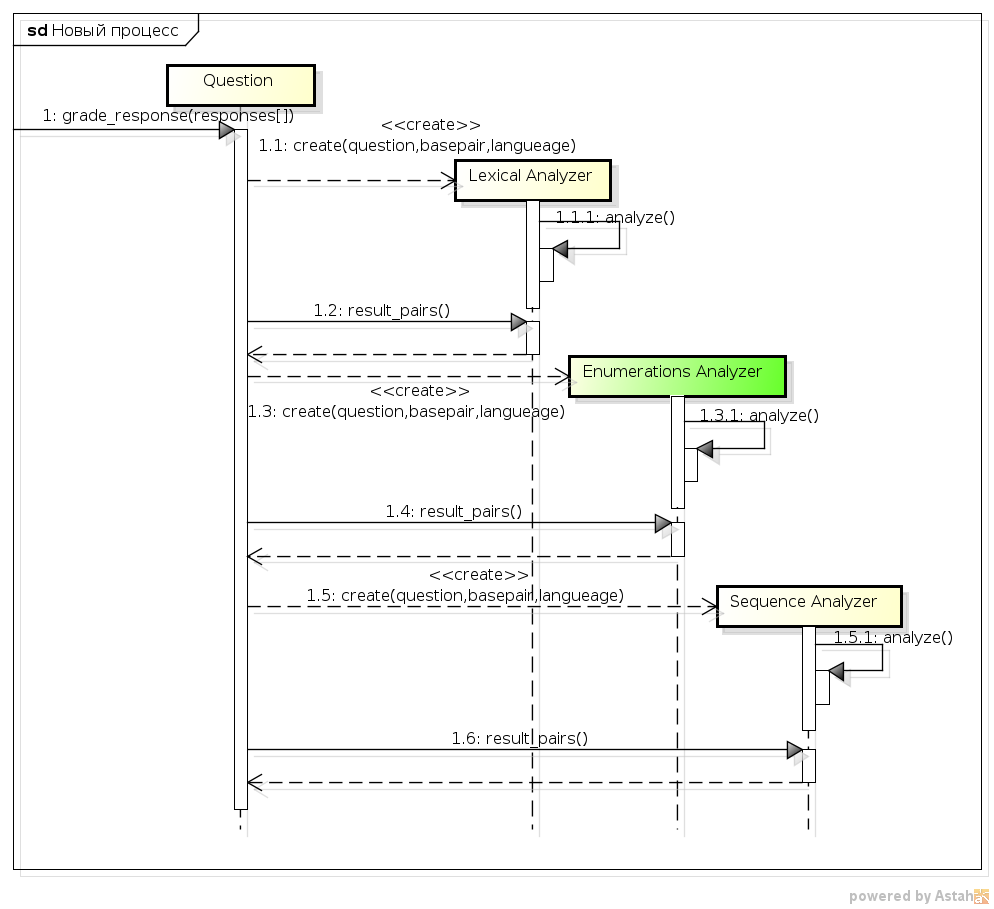
\includegraphics[width = \linewidth]{tzsequence.png}
\caption{Диаграмма последовательности}\label{sequence}
\end{figure}
\par Зеленым выделены реализуемые компоненты.
\appendixtz{Макет графического интерфейса}
На рисунке~\ref{gui} представлен графический интерфейс:
\begin{enumerate}
    \item 1 - поле редактирования эталонного ответа; 
    \item 2 - графическое обозначение элемента;
    \item 3 - иконка удаления элемента перечисления;
    \item 4 - список перечислений;
    \item 5 - кнопка добавления перечисления;
    \item 6 - кнопка удаления перечисления;
\end{enumerate}
\begin{figure} 
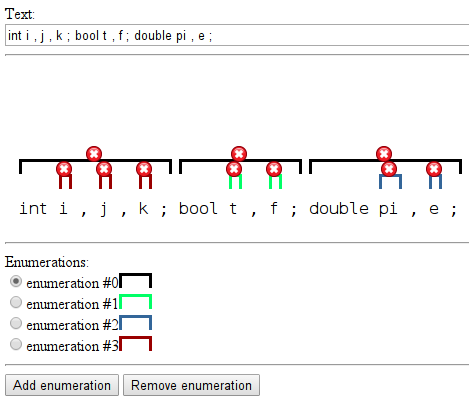
\includegraphics[width = \linewidth]{gui.png}
\caption{Макет графического интерфейса}\label{gui}
\end{figure}
\par Изменение границ элемента происходит путем перетаскивания правой или левой вертикальной границы обозначения элемента.

\appendixtz{Тестовый пример для графического интерфейса}
\par Ход теста: 
\begin{enumerate}
    \item создать вопрос типа CorrectWriting, для этого:
        \begin{enumerate}
            \item открыть Question Bank;
            \item нажать на кнопку "Добавить вопрос"
            \item выбрать тип вопроса "CorrectWriting";
            \item добавить название вопроса;
            \item включить поля "Analysis of enumerations" и "Token sequence analysis";
            \item выключить поле "Typo analysis";
            \item ввести эталонный ответ: "int integer = 3, variable = integer; bool isFind, endOfGame;"
            \item вызвать графический интерфейс редактирования перечислений;
            \item убедиться, что "integer = 3" и "variable = integer" являются элементами одного перечисления, а "isFind" и "endOfGame" элементами другого;
            \item удалить перечисление, элементом которого является "variable = integer";
            \item добавить новое перечисление;
            \item добавить новому перечислению элементы "int integer = 3, variable = integer" и "bool isFind, endOfGame";
            \item добавить описание каждой лексеме правильного ответа;
            \item сохранить вопрос
        \end{enumerate}
    \item открыть предварительный просмотр ранее созданного вопроса;
    \item в открышемся окне в поле ответа ввести строку: "bool endOfGame, isFind; int variable = integer, integer = 3;";
    \item нажать кнопку "оценить";
    \item убедиться, что ошибки связано с перемещением лексем "variable", "=", "integer" и ",";
    \item закрыть окно предварительного просмотра.
\end{enumerate}
\appendixtz{Тестовый пример для процесса оценивания}
\par Ход теста: 
\begin{enumerate}
    \item открыть вопрос типа CorrectWriting, для этого:
        \begin{enumerate}
            \item открыть Question Bank;
            \item выбрать вопрос с названием "Enumerate analyzer test";
            \item открыть редактирование вопроса;
        \end{enumerate}
    \item убедиться, что включено поле "Analysis of enumerations" и "Token sequence analysis";
    \item убедиться, что выключено поле "Typo analysis";
    \item убедиться, что эталонный ответ только один и его текст эквивалентен "struct  MyNiceStructure \{ int  FirstField;  long Padding;  char  SmallPart; \} DefaultValue;";
    \item закрыть редактирование вопроса;
    \item открыть предварительный просмотр вопроса;
    \item в открывшемся окне в поле ответа ввести строку: "struct MyNiceStructure \{long Padding; char SmallPart; int FirstField;\} DefaultValue;";
    \item нажать кнопку "оценить" и убедиться что в ответ оценен на максимальный бал;
    \item закрыть окно предварительного просмотра.
\end{enumerate}
\end{document}
